\documentclass[tikz]{standalone}

\usetikzlibrary{shapes}
\usetikzlibrary{calc} 
\usetikzlibrary{positioning}


% This bascially automates a \newcommand{<name>}{} to ensure
% that a command with the given <name> does not already exist
\providecommand*{\pgfmathsetnewmacro}[2]{%
    \newcommand*{#1}{}% Error if already defined
    \pgfmathsetmacro{#1}{#2}%
}%


\begin{document}
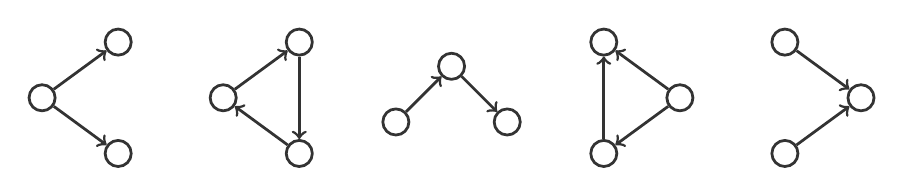
\begin{tikzpicture}[black!80, line width = 1pt]

    \coordinate (O) at (0,0);

    %\draw[help lines, opacity = 0.1] (-4,-4) grid (4,4);

    \begin{scope}[on grid, xshift = -5.2cm]
        
        \node (O) at (0,0) [circle, draw, fill = white] {};
              
        \node (N1) [circle, draw, fill = white, above right=1 of O.south east] {};
        \node (N2) [circle, draw, fill = white, below right=1 of O.north east] {};

        \draw[->] (O) -- (N1);
        \draw[->] (O) -- (N2);


        % \node (notation1) [below right = of O, yshift = -1cm ] {$\left\langle 1,2 \right\rangle$};
    \end{scope}
        
    \begin{scope}[on grid, xshift = +5.2cm]
        
        \node (O) at (0,0) [circle, draw, fill = white] {};
              
        \node (N1) [circle, draw, fill = white, above left=1 of O.south west] {};
        \node (N2) [circle, draw, fill = white, below left=1 of O.north west] {};

        \draw[->] (N1) -- (O);
        \draw[->] (N2) -- (O);

        % \node (notation1) [below left = of O, yshift = -1cm ] {$\left\langle 2,1 \right\rangle$};
    \end{scope}

    \begin{scope}[on grid, xshift = +2.9cm]
        
        \node (O) at (0,0) [circle, draw, fill = white] {};
              
        \node (N1) [circle, draw, fill = white, above left=1 of O.south west] {};
        \node (N2) [circle, draw, fill = white, below left=1 of O.north west] {};

        \draw[<-] (N1) -- (O);
        \draw[->] (O) -- (N2);
        \draw[->] (N2) -- (N1);

        % \node (notation1) [below left = of O, yshift = -1cm ] {$\left\langle 2,1 \right\rangle$};
    \end{scope}
    \begin{scope}[on grid, xshift = -2.9cm]
        
        \node (O) at (0,0) [circle, draw, fill = white] {};
              
        \node (N1) [circle, draw, fill = white, above right=1 of O.south east] {};
        \node (N2) [circle, draw, fill = white, below right=1 of O.north east] {};

        \draw[<-] (N1) -- (O);
        \draw[<-] (O) -- (N2);
        \draw[<-] (N2) -- (N1);

        % \node (notation1) [below left = of O, yshift = -1cm ] {$\left\langle 2,1 \right\rangle$};
    \end{scope}
    
    
    \begin{scope}[on grid, yshift = +0.4cm]
        
        \node (O) at (0,0) [circle, draw, fill = white] {};
              
        \node (N1) [circle, draw, fill = white, below right=1 of O] {};
        \node (N2) [circle, draw, fill = white, below left=1 of O] {};

        \draw[<-] (N1) -- (O);
        \draw[<-] (O) -- (N2);

        % \node (notation1) [below left = of O, yshift = -1cm ] {$\left\langle 2,1 \right\rangle$};
    \end{scope}
    
\end{tikzpicture}
\end{document}